% Benchmark Calibration Table
% !TEX TS-program = pdflatex
% !TEX options = -shell-escape -synctex=1 -interaction=nonstopmode -file-line-error "%DOC%"
% 
\documentclass[margin=10pt, convert={outname=../images/branchExample4}]{standalone}    
\usepackage{pgfplots, pgf, natbib, textpos,ragged2e, colortbl, cancel, array, pgfplotstable, amsmath} 

\usetikzlibrary{calc, positioning, backgrounds, decorations.markings, external, arrows.meta, arrows, shapes, snakes, fit}
\usetikzlibrary{shapes,snakes}
\pgfplotsset{tick label style={font=\small}, label style={font=\small}, legend style={font=\small}, compat= newest}

\definecolor{UBCblue}{RGB}{12, 35, 68} 
\definecolor{UBClblue}{RGB}{0, 85, 183}
\definecolor{UBCgreen}{RGB}{88, 162, 41} 
\definecolor{UBCred}{RGB}{203, 29, 56}
\definecolor{UBCgrey}{RGB}{116, 145, 163}


\begin{document} 
	%<*tikzPic>
	
	\pgfplotsset{scale only axis, width=0.85\textwidth, height=0.5\textwidth}
	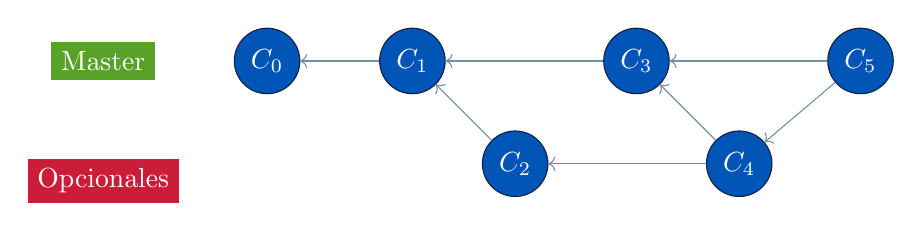
\begin{tikzpicture}[]
		
		% Master
		\node[shape=rectangle, draw=UBCgreen, fill=UBCgreen] (master) at (0,0) {\color{white}Master};
		\node[shape=circle, draw=UBCblue, fill=UBClblue, right = 1cm of master] (c0) {\color{white}$C_{0}$};
		\node[shape=circle, draw=UBCblue, fill=UBClblue, right = 1cm of c0] (c1) {\color{white}$C_{1}$};
		\node[shape=circle, draw=UBCblue, fill=UBClblue, right = 2cm  of c1] (c3) {\color{white}$C_{3}$};
		\node[shape=circle, draw=UBCblue, fill=UBClblue, right = 2cm  of c3] (c5) {\color{white}$C_{5}$};
		\path[UBCgrey, ->] (c1) edge (c0);
		\path[UBCgrey, ->] (c3) edge (c1);
		\path[UBCgrey, ->] (c5) edge (c3);
		
		
		% Opcionales
		\node[shape=rectangle, draw=UBCred, fill=UBCred, below = 1cm of master] (opcionales) {\color{white}Opcionales};
		\node[shape=circle, draw=UBCblue, fill=UBClblue, below right = 1cm  of c1] (c2) {\color{white}$C_{2}$};
		\node[shape=circle, draw=UBCblue, fill=UBClblue, right = 2cm  of c2] (c4) {\color{white}$C_{4}$};
		\path[UBCgrey, ->] (c2) edge (c1);
		\path[UBCgrey, ->] (c4) edge (c2);
		\path[UBCgrey, ->] (c4) edge (c3);
		\path[UBCgrey, ->] (c5) edge (c4);
	\end{tikzpicture}%
	%</tikzPic>
	
\end{document}
